% !TEX root = ../main.tex
%\MY{use anonymous template, with line numbers and page numbers}
\section{Introduction}
Nowadays, the rising prevalence of mental health-related issues presents a significant and growing threat to global public health~\citep{evans2018socioeconomic}. Despite their widespread impact, these challenges are often underestimated due to societal stigma and a lack of public awareness~\citep{pirina2018identifying}. The pervasive specter of mental illness, especially depression, poses substantial challenges on a global scale, with the World Health Organization (WHO) estimating that 3.8\% of the global population experiences depression~\citep{who2023depression}. 
% This issue is further emphasized in regions like China, where the prevalence of depression is notably high at around 6.9\%, underscoring the escalating mental health concerns within the nation~\citep{huang2019prevalence}.

% CSY: 感觉这里有点怪,一直以来大家都很关注mental health,并不是大模型出来后才关注的;可以说大模型的出现,为mental health领域的一些长期存在的问题提供了新的解决思路;然后讲大模型的优点balabala(√)
In the face of the escalating global public health challenge posed by mental health issues, an increasing cohort of researchers has redirected substantial efforts towards this critical domain ~\citep{Lamichhane2023chatgptapp}. The advent of large language models (LLMs) has emerged as a transformative force, offering novel solutions to persistent challenges within the field of mental health. Notable models such as ChatGPT~\citep{schulman2022chatgpt}, LLaMA~\citep{touvron2023llama}, and Vicuna~\citep{chiang2023vicuna} have made substantial strides in Natural Language Processing (NLP). These models leverage extensive pretraining data and massive neural networks, achieving commendable results on standard NLP benchmark tests. In the specific domain of mental health, these LLMs have shown promising applications~\citep{xu2023leveraging, Lamichhane2023chatgptapp}. Concurrently, researchers have recognized the unique demands of the mental health domain and have introduced specialized LLM explicitly designed for mental health applications~\citep{yang2023mentallama}.

    \begin{figure*}[th]
        \centering
        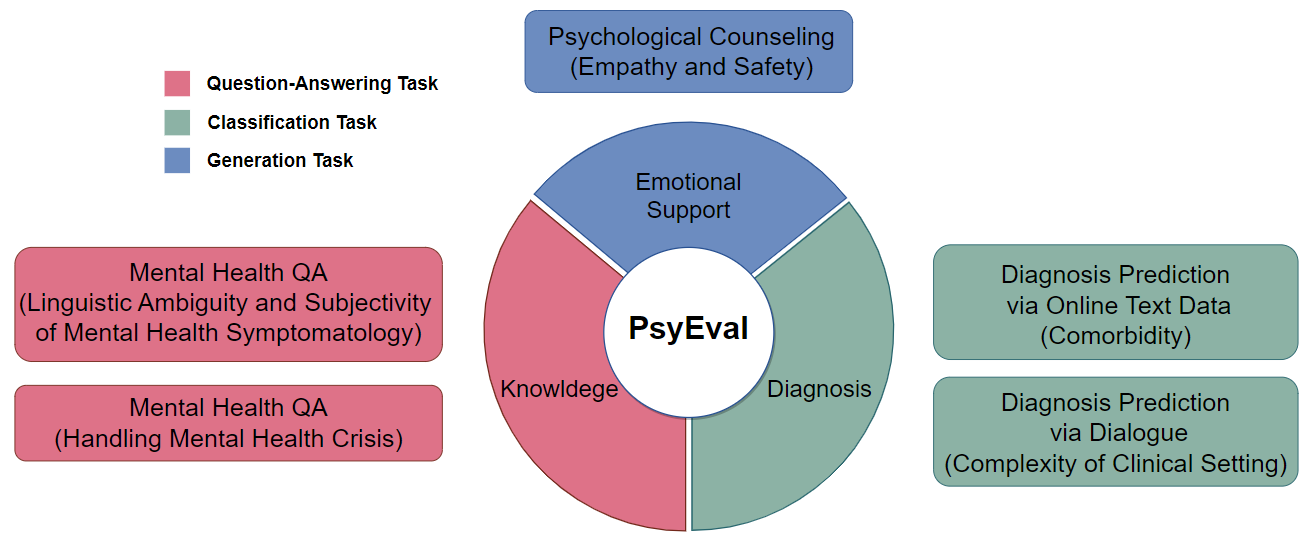
\includegraphics[width=0.8\textwidth]{Figure/PsyEval.png}
        \caption{Overview diagram of PsyEval}
    \end{figure*}
    
The application of LLMs in mental health is a growing area with distinctive challenges. Unlike other fields, assessing LLMs for mental health requires a careful approach due to the subtle and highly subjective nature of symptoms, which vary widely among individuals~\citep{taschereau2022putting}.
%\MY{add a ref here} 
In this domain, models are required to resemble a professional psychologist, possessing substantial knowledge in mental health, diagnostic capabilities for illnesses, and the ability to exhibit empathy and ethical conduct~\citep{iaap_iupsys_2016}.
%\KZ{Not sure what are the emergency situations? All of the above requirements should be reflected in our benchmark tests.}
While various benchmarks evaluate LLMs in general language tasks (e.g., C-EVAL~\citep{huang2023ceval}, AGIEval~\citep{zhong2023agieval}, MMLU~\citep{hendrycks2021measuring}), there is a notable absence of a dedicated and comprehensive benchmark for the mental health. Existing benchmarks like Mental-LLM~\citep{xu2023leveraging} and DialogueSafety~\citep{qiu2023benchmark}, while relevant, focus on specific aspects and lack a holistic evaluation of LLMs in addressing the diverse challenges of mental health data and scenarios. Thus, there is a clear need for a specialized benchmark to thoroughly assess LLM performance in the unique complexities of the mental health domain. %\KZ{The sentences above are wordy and can be simplified.}

To address this gap, we introduce PsyEval, a meticulously crafted benchmark designed to comprehensively evaluate the performance of LLMs in mental health-related tasks. 

\paragraph{Design Philosophy of PsyEval} PsyEval aims to provide a nuanced assessment of the strengths and limitations of LLMs. Qualified mental health professionals must possess \textit{extensive domain knowledge}, \textit{diagnostic acumen}, and \textit{emotional support capabilities}. PsyEval evaluates LLMs across these three dimensions. Moreover, when setting the tasks, we carefully considered the specific characteristics of the mental health domain:
\begin{itemize}
    \item Psychiatric symptoms are subtly expressed and challenging to articulate due to \textbf{linguistic ambiguity and subjectivity}. Understanding this nuanced expression of symptoms is crucial for LLM in mental health area, which demands substantial domain knowledge. Hence, we included a mental health QA task to assess the model's grasp of fundamental mental health knowledge.
    \item \textbf{Mental health crisis} can lead to severe consequences hence safety requirement and emergency protocol is important. Generally, practitioners must follow General Principles~\citep{apa_ethical_principles_2002} of mental health support, which require them take care to do no harm. PsyEval contains a task focusing on mental health crisis.
    \item \textbf{Comorbidity} of several mental disorders is common in clinical practice. Our benchmark goes beyond traditional setups that focus on the detection of one mental disorder. It includes tasks for simultaneously detecting multiple disorders, assessing the model's ability to understand both commonality and distinction among different disorders. 
    \item Individuals with mental health conditions often lack self-awareness and may not accurately judge their own situation. In actual diagnostic scenarios, patients may present with preconceived notions of having a particular condition, leading to a mismatch between their expressed language and the reality. In order to address the \textbf{complexity of diagnostic environments} in real-world scenarios, we designed a task involving the prediction of diagnoses in simulated doctor-patient dialogues.
    \item Mental health patients often experience feelings of shame, contributing to emotional resistance or reluctance to fully disclose thoughts during consultation and diagnostic processes. This requires therapists to adopt specific strategies and possess empathy. PsyEval includes a task simulating mental health counselors providing emotional support to seekers and assessing the \textbf{empathy} in the model's output. Additionally, we emphasize that the model's outputs must ensure \textbf{safety}, avoiding any adverse physical or psychological impact on the seeker.
     %\KZ{I don't know why u call it safety understanding. To ensure the model understands safety? I think you want the model to respond ethically and responsibly, not to understand safety or act safely. The safest thing to do is not saying anything!}
\end{itemize}

% \begin{table*}[t]
%     \centering
%     \begin{tabular}{c c c}
%          \hline
%          Task & Capability & Challenge \\
%          \hline
%          Mental health QA & possess the necessary knowledge & linguistic ambiguity and subjectivity of Mental health diseases \\
%          Diagnosis Prediction via Online Text Data & diagnosis capability & disease co-occurrence \\
%          Diagnosis Prediction via Dialogue & diagnosis capability & patients lack self-awareness \\
%          Therapeutic Conversations & emotion support capability & resolve emotional resistance \\
%          Empathy Capability & exhibit empathy & \\
%          Safety Awareness & exhibit ethical & ethical consideration \\
%          \hline
%     \end{tabular}
%     \caption{Caption}
%     \label{tab:my_label}
% \end{table*}

% CSY: 我觉得这里的五点要和你的benchmark设置对应起来,就是为什么要挑这些任务【主旨:挑的任务可以很好地evaluate到mental health 领域特别需要在意的部分的模型能力(可以在这一段的开头亮明)】。具体分析比如,
% 1. ethical concern对于mental health 领域非常重要,所以benchmark必须包括ethical的部分(我看到你写了)
% 2. mental illness co-occur普遍,所以我们的benchmark里包含的任务是多疾病的共同检测,而非传统的单疾病检测
% 3. mental health 领域患者的耻感和抗拒导致医生问诊/咨询时必须有同理心,所以我们的benchmark里有empathy部分的评估
% 4. 可以自己再想想
%(有可能的话,感觉Figure 1可以把这五点和任务对应上,都体现在图里?字太多的话就算了)(√)

% By considering these specific challenges, PsyEval aims to provide a comprehensive evaluation of LLMs' capabilities in addressing the complexities of mental health data and scenarios.

% summary, the contributions of this work are as follows: (1) We propose a new benchmark PsyEval to meet the need for systematic evaluations of LLMs in mental health. (2) We conduct abundant experiments on a total of 6 sub-tasks to comprehensively evaluate 8 up-to-date LLMs, using various prompts for different tasks, including answer-only, few-shot, and chain-of-thought (CoT). (3) We summarize the exposed problems in experiments, proving guidance for the evolution of LLMs.

%CSY_v2: 也许在introduction最后写一个简单的takeaways(包括这篇paper所有的结论性的东西)让读者一目了然?(√)
%\paragraph{Summary of findings} After benchmarking various LLMs using PsyEval, we get the following observations: (1) GPT-4 demonstrated commendable proficiency in mental health knowledge, matching psychiatric professional's capabilities. (2) However, in complex tasks such as identifying multiple disorders and diagnosing depression through doctor-patient dialogues, all models struggled to achieve satisfactory performance. (3) Models equipped with larger context windows, designed to handle extensive input texts in these tasks, exhibited relatively superior performance. (4) All models exhibited a limited understanding of empathy and dialogue safety in mental health counseling scenarios, highlighting the need for advancements in comprehending human emotions and situations. %\KZ{When you said understanding of empathy and safety, you mean the model doesn't understand the word empathy and safety in the prompt? I think they do. They just don't know how to perform it. So be careful with the word `` understanding''. And what do you mean by situations specifically?}

%\KZ{Generally speaking, this paper is wordy at places, and repeats itself.}



% The results reveal a notable disparity in the models' performance across various mental health tasks. GPT-4 demonstrated a commendable proficiency in grasping mental health knowledge, reaching a level comparable to human capabilities. However, when faced with challenges like identifying multiple disorders in social media posts and diagnosing depression in simulated doctor-patient dialogues, all models fell short of achieving satisfactory levels of accuracy.Significantly, models equipped with larger context windows, designed to handle extensive input texts in these tasks, exhibited relatively superior performance. This underscores the critical role of addressing context window limitations in mental health-related assignments. The intricate nature of mental health discussions and diagnostic processes demands a broader contextual understanding, which larger context windows appear to facilitate.Furthermore, the models displayed a limited grasp of empathy and dialogue safety in the context of mental health counseling scenarios. This deficiency emphasizes the need for advancements in the models' comprehension of nuanced emotional nuances and the maintenance of safe, supportive dialogue environments in mental health-related conversations.Notably, in tasks related to diagnosing depression in simulated real-life doctor-patient dialogues, simulating psychological counseling, and understanding dialogue safety, models specifically trained for the Chinese language showcased superior performance. This underscores the indispensability of language-specific training in the realm of psychological counseling and diagnosis, emphasizing the need for models to be adept in the linguistic nuances of the target language for enhanced efficacy.



%CSY: mental health领域本身和其它有什么不一样%
%   1.精神疾病症状的语言表达具有模糊性和主观性,且比较微妙,难以完全用语言表达出来,同样的症状不同的人表达差异也比较大
%   2.精神疾病经常出现共病,导致疾病标签之间可能存在交叉
%   3.精神疾病患者往往具有耻感,在咨询、诊断过程中可能存在抗拒情绪或不愿完全袒露自己的想法
%   4.精神疾病领域对ethical concern相当关注
%   5.精神疾病领域数据难以收集
